
\documentclass[english]{article}
%%%%%%%%%%%%%%%%%%%%%%%%%%%%%%%%%%%%%%%%%%%%%%%%%%%%%%%%%%%%%%%%%%%%%%%%%%%%%%%%%%%%%%%%%%%%%%%%%%%%%%%%%%%%%%%%%%%%%%%%%%%%
\usepackage{latexsym,amsmath,amssymb,amsfonts,fullpage}
\usepackage{gensymb}
\usepackage{tikz}
\usetikzlibrary{arrows,shapes}

\begin{document}

\begin{center}
{\textbf{MEAM 620 Homework 1}} \\
Due: Monday, January 26, 11:59pm 
\end{center}






\paragraph{1.}

Show (or disprove) that the $A^*$ algorithm reduces (is equivalent in terms of computations) to: 
(a) Dijkstra's algorithm if $h=0$; and (b) the depth-first search algorithm if $h$ is the depth of the graph. 

\begin{enumerate}
\item[(a)] Dijkstra's algorithm has the same structure as $A^*$, except it chooses the node $s$ with the minimum cost incurred thus far. $A^*$ chooses the node $s$ with the minimum $f(s)$, but $f(s) = g(s) + h(s)$ where $g(s)$ is the cost incurred thus far. Therefore if $h(s) = 0$ for all $s$ then $f(s) = g(s)$ which is the same cost function that Dijkstra chooses from.
\item[(b)] No this does behave the same way as depth-first search. Consider the simple graph: 

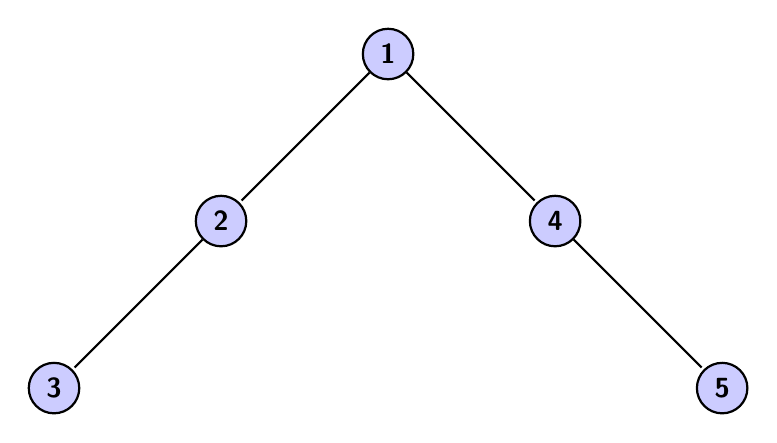
\begin{tikzpicture}[->,>=stealth',shorten >=1pt,auto,node distance=3cm,
  thick,main node/.style={circle,fill=blue!20,draw,font=\sffamily\bfseries}] %[shorten >=1pt,node distance=2cm,auto] 
   \node[main node] (a)   {1}; 
   \node[main node] (b) [below left of=a] {2}; 
   \node[main node] (c) [below left of=b] {3};
   \node[main node] (d) [below right of=a] {4};
   \node[main node] (e) [below right of=d] {5};
    \path[-] 
    (a) edge node {} (b)
        edge node {} (d)
    (b) edge node {} (c)
    (d) edge node {} (e);
\end{tikzpicture}

A simple DFS search starting from 1 would give the node order 1,2,3,4,5. If we used $A^{*}$ with the heuristic described, we would first select 2 as before. However on choosing our next node, $g(4) + h(4) = 1 + 1 = 2$ and $g(3) + h(3) = 2 + 2 = 4$ so we would choose 4 next, and continuing this way we would get the node order 1,2,4,3,5. This is not a DFS search and therefore we have provided a counter-example, disproving the claim.

\end{enumerate}

\paragraph{2.}

(a) Show that the set of rotation matrices forms a group. (b) Is the set of orthogonal matrices a group? Explain. 
\begin{enumerate}
\item[(a)] It does form a group, if we consider matrix multiplication as the operator. A matrix $R$ is a rotation matrix if and only if $R^\top R = R R^\top = I$ and $\mathrm{det}(R) = +1$.
	\begin{enumerate}
	\item \textbf{Closure}: If $R_1$ and $R_2$ are both rotation matrices then $R_1 R_2$ is also a rotation matrix. The proof is as follows:
		\begin{align*}
			(R_1 R_2)^\top (R_1 R_2)
					&=\; R_2^\top R_1^\top R_1 R_2 & \textrm{(Transpose of matrix multiplication)} \\
					&=\; R_2^\top I R_2 & \textrm{(Definition of rotation matrix)} \\
					&=\; R_2^\top R_2 & \textrm{(Definition of identity)} \\
					&=\; I & \textrm{(Definition of rotation matrix)} \\
		\end{align*}
		Similarly for the other way, $ (R_1 R_2) (R_1 R_2)^\top = R_1 R_2 R_2^\top R_1^\top = R_1 R_1^\top = I$. Now the determinant of $R_1 R_2$ is $det(R_1 R_2) = det(R_1) det(R_1) = (1)^2 = 1$, so it still has positive unit determinant.
		Therefore $R_1 R_2$ is also a rotation matrix so the group is closed under matrix multiplication
	\item \textbf{Associativity}: Matrix multiplication is associative, so this follows directly from that.
	\item \textbf{Existence of Identity}: There is an identity element, namely $I$. Clearly $I^\top I = I I^\top = I$, so it is a rotation matrix, and for any matrix $A$, including rotation matrices, $A I = I A = A$, so it is the identity element for the matrix multiplication operator (hence identity matrix).
	\item \textbf{Existence of inverse element}: Since $I$ is the identity element, and by definition $R^\top R = R R^\top = I$, $R$ has an inverse element, namely $R^\top$.
	\end{enumerate}
\item[(b)] Orthogonal matrices are exactly the same as rotation except that there is no constraint on the determinant, it can be either $+1$ or $-1$. This changes the determinant argument from the closure argument from the group to $R_1 R_2$ is $det(R_1 R_2) = det(R_1) det(R_1) \in \{(+1)(+1), (-1)(+1), (+1)(-1), (-1)(-1)\} = \{+1,-1\}$, so it is still in the set of orthogonal matrices. So the above argument still holds for orthogonal matrices. 
 
\end{enumerate}

\paragraph{3.}

Write down the appropriate number of  independent constraints on the 9 elements of a rotation matrix: 
\[
{\bf R} = \begin{bmatrix} 
			R_{11} & R_{12} & R_{13}  \\
			R_{21} & R_{22} & R_{23}  \\
			R_{31} & R_{32} & R_{33}
		\end{bmatrix}
\]

% Some of these constraints are not independent. Reduce them
\begin{itemize}
\item Unit norm column vectors
\begin{itemize}
\item[1.] $ R_{11}^2 + R_{12}^2 + R_{13}^2 = 1$
\item[2.] $ R_{21}^2 + R_{22}^2 + R_{23}^2 = 1$
\item[3.] $ R_{31}^2 + R_{32}^2 + R_{33}^2 = 1$
\end{itemize}
\item Orthogonal column vectors
\begin{itemize}
\item[4.] $ R_{11} R_{12} + R_{21} R_{22} + R_{31} R_{32} = 0$
\item[5.] $ R_{11} R_{13} + R_{21} R_{23} + R_{31} R_{33} = 0$
\item[6.] $ R_{12} R_{13} + R_{22} R_{23} + R_{32} R_{33} = 0$
\end{itemize}
\item Positive unit determinant
\begin{itemize}
\item[7.] $\mathrm{det}(R) = R_{11}(R_{22}R_{33} - R_{23}R_{32}) - R_{12}(R_{21}R_{33} - R_{23}R_{31}) + R_{13}(R_{21}R_{32} - R_{22}R_{31})= +1$
\end{itemize}
\end{itemize}

\paragraph{4.} 

For a rotation matrix as defined in Problem 3, prove that: 
\[
R_{11} = \begin{vmatrix}
R_{22} & R_{23}  \\
R_{32} & R_{33} \end{vmatrix}
\]

Consider the determinant of a rotation matrix:

\[ \mathrm{det}(R) = R_{11}(R_{22}R_{33} - R_{23}R_{32}) - R_{12}(R_{21}R_{33} - R_{23}R_{31}) + R_{13}(R_{21}R_{32} - R_{22}R_{31})= +1 \]
\[ \implies R_{11}(R_{22}R_{33} - R_{23}R_{32}) + R_{12}(R_{23}R_{31} - R_{21}R_{33}) + R_{13}(R_{21}R_{32} - R_{22}R_{31})= +1 \]

Let $a = R_{22}R_{33} - R_{23}R_{32}$, $b = R_{23}R_{31} - R_{21}R_{33}$, and $c = R_{21}R_{32} - R_{22}R_{31}$. Then:
\[ R_{11}(a) + R_{12}(b) + R_{13}(b) = +1 \implies
\begin{bmatrix}
	R_{11} \\
	R_{12} \\
	R_{13}
\end{bmatrix} \cdot \begin{bmatrix}
	a \\
	b \\ 
	c
\end{bmatrix} = 1 \] 

So by the definition of dot product, this equals $||(a,b,c)^\top||\cos \theta$ (constraint 1 shows the left vector is unit norm). If we can prove $(a,b,c)^\top$ is unit norm, we will show that $(a,b,c) = (R_{11},R_{12},R_{13})$ by constraint 1 of rotation matrices. We show that here, using other properties of the rotation matrix (labelled in previous problem)
\begin{align*}
 &\; a^2 + b^2 + c^2 \\
=&\; (R_{22}R_{33} - R_{23}R_{32})^2 + (R_{23}R_{31} - R_{21}R_{33})^2 + (R_{21}R_{32} - R_{22}R_{31})^2 \\
=&\; R_{22}^2R_{33}^2 + R_{23}^2R_{32}^2 - 2 R_{22}R_{33}R_{23}R_{32}  \\
 &\;\; + R_{23}^2R_{31}^2 + R_{21}^2R_{33}^2 - 2R_{23}R_{31}R_{21}R_{33} \\
 &\;\; + R_{21}^2R_{32}^2 + R_{22}^2R_{31}^2 - 2R_{21}R_{32}R_{22}R_{31} \\
=&\; R_{21}^2(R_{32}^2 + R_{33}^2) + R_{22}^2(R_{31}^2 + R_{33}^2) + R_{23}^2(R_{31}^2 + R_{32}^2) \\
 &\;\;  - (2R_{23}R_{31}R_{21}R_{33} + 2 R_{22}R_{33}R_{23}R_{32} + 2R_{21}R_{32}R_{22}R_{31}) \\
=&\; R_{21}^2(1 - R_{31}^2) + R_{22}^2(1 - R_{32}^2) + R_{23}^2(1 - R_{33}^2) \\
 &\;\;  - (2R_{23}R_{31}R_{21}R_{33} + 2 R_{22}R_{33}R_{23}R_{32} + 2R_{21}R_{32}R_{22}R_{31}) & \textrm{(Constraint 3.)} \\
=&\; R_{21}^2  + R_{22}^2 + R_{23}^2 - ((R_{21}R_{31})^2 + (R_{22}R_{32})^2 + (R_{23}R_{33})^2 \\
 &\;\;\; + 2(R_{23}R_{31})(R_{21}R_{33}) + 2(R_{22}R_{33})(R_{23}R_{32}) + 2(R_{21}R_{32})(R_{22}R_{31})) \\
=&\; R_{21}^2  + R_{22}^2 + R_{23}^2 - (R_{21}R_{31} + R_{22}R_{32} + R_{23}R_{33})^2 \\
=&\; 1 - (0)^2 & \textrm{(Constraint 2 and property below)} \\
=&\; 1 \\
\end{align*}

The second to last step uses the fact that the rows are orthonormal as well. Properties 1-6 of rotation matrices can be summarized as $R^\top R = I$ in matrix notation. Showing the rows are orthonormal is equivalent to showing $R R^\top = I$, which we can prove simply:
\[ R^\top R = I \implies R R^\top R R^\top = R R^\top \implies R R^\top = (R R^\top)^{-1}(R R^\top)  = I \]
And we can invert $R R^\top$ since $det(R R^\top) = det(R) det(R^\top) = det(R)^2 = 1$.

That concludes the proof.

\paragraph{5.}

Consider a $2 \times 2$ rotation matrix which takes the form
\[
{\bf R} = \begin{bmatrix} \cos \theta & -\sin \theta  \\
\sin \theta  & \cos \theta \end{bmatrix}, 
\]
and another fixed but arbitrarily chosen $2 \times 2$ rotation matrix {\bf S}. 
Show that ${\bf R}^{-1}$ is a continuous function of ${\bf R}$ and {\bf RS} is a continuous function of {\bf R}. 

\paragraph{ }

To show continuity, we will show that  ${\bf R}(\theta + d\theta)^{-1}R(\theta) \rightarrow I$ as $d\theta \rightarrow 0$, and similarly ${\bf R}(\theta + d\theta)S \rightarrow {\bf R}(\theta)S$ as $d\theta \rightarrow 0$. This is equivalent to saying that $ \lim_{R_1 \rightarrow R} f(R_1) = R$, which proves continuity. We show they approach each other by showing that the Frobenius norm of their difference goes to zero.

One more note before the proofs. We have
\[
{\bf R}(\theta) = \begin{bmatrix} \cos \theta & -\sin \theta  \\
\sin \theta  & \cos \theta \end{bmatrix} 
\]
Consider an element with a small change in rotation
\begin{align*}
{\bf R}(\theta + d\theta)
	&=\; \begin{bmatrix}
			\cos(\theta + d\theta) & -\sin(\theta + d\theta) \\
			\sin(\theta + d\theta) & \cos(\theta + d\theta)
		\end{bmatrix} \\
	&=\; \begin{bmatrix}
			\cos(\theta)\cos(d\theta) - \sin(\theta)\sin(d\theta) & -\sin(\theta)\cos(d\theta) - \cos(\theta)\sin(d\theta) \\
			\sin(\theta)\cos(d\theta) + \cos(\theta)\sin(d\theta) & \cos(\theta)\cos(d\theta) - \sin(\theta)\sin(d\theta)
		\end{bmatrix} \\
	&=\; \begin{bmatrix}
			\cos(\theta) & -\sin(\theta) \\
			\sin(\theta) & \cos(\theta)
		\end{bmatrix} \begin{bmatrix}
			\cos(d\theta) & -\sin(d\theta) \\
			\sin(d\theta) & \cos(d\theta)
		\end{bmatrix} \\
	&=\; {\bf R}(\theta){\bf R}(d\theta)
\end{align*}
This property will be assumed for the proofs. 

\begin{enumerate}

\item[(a)] So we look at the multiplication of ${\bf R}(\theta + d\theta)^{-1} = {\bf R}(d\theta)^\top{\bf R}(\theta)^\top$ with ${\bf R}(\theta)$. The Frobenius norm of this is:

\begin{align*}
&\; \left| \left| {\bf R}(d\theta)^\top{\bf R}(\theta)^\top {\bf R}(\theta) - {\bf R}(\theta)^\top {\bf R}(\theta) \right| \right|_F \\
=&\; \left| \left| {\bf R}(d\theta)^\top - I \right| \right|_F  \\
=&\; \left| \left| \begin{bmatrix}
			\cos(d\theta) - 1 & \sin(d\theta) \\
			-\sin(d\theta) & \cos(d\theta) - 1
		\end{bmatrix} \right| \right|_F \\
=&\; (\cos(d\theta) - 1)^2 + (\sin(d\theta))^2 + (-\sin(d\theta))^2 + (\cos(d\theta) - 1)^2 \\
=&\; 2(\cos^2(d\theta) - 2\cos(d\theta) + 1) + 2\sin^2(d\theta) \\
=&\; 2(\cos^2(d\theta) + \sin^2(d\theta)) + 2 - 4\cos(d\theta) \\
=&\; 4(1 - \cos(d\theta))
\end{align*}

Since $\cos(d\theta) \rightarrow 1$ as $d\theta \rightarrow 0$, this term goes to zero.

\item[(b)] Now we consider the product ${\bf R}(\theta + d\theta) {\bf S} = {\bf R}(\theta) {\bf R}(d\theta) {\bf S}$ and its appropriate norm of the difference:
\begin{align*}
    &\; ||{\bf R}(\theta) {\bf R}(d\theta) {\bf S} - {\bf R}(\theta) {\bf S}||_F \\
  = &\; ||{\bf R}(\theta)({\bf R}(d\theta) - I) {\bf S}||_F \\
\le &\; ||{\bf R}(\theta)||_F ||({\bf R}(d\theta) - I)||_F ||{\bf S}||_F & \textrm{(Properties of Frobenius Norm)} \\
  = &\; 4 ||({\bf R}(d\theta) - I)||_F  & \textrm{(Frobenius norm of rotation matrices)} \\
  = &\; 16 (1 - \cos(d\theta))  & \textrm{(From part (a))} \\
\end{align*}

As said in part (a), $\cos(d\theta) \rightarrow 1$ as $d\theta \rightarrow 0$, so this whole term goes to zero. To prove the 4th step, we show the Frobenius norm of any 2 by 2 rotation matrix is 2:
\begin{align*}
&\; \left| \left| \begin{bmatrix}
			\cos(\theta) & -\sin(\theta) \\
			\sin(\theta) &  \cos(\theta)
		\end{bmatrix} \right| \right|_F \\
=&\; (\cos(\theta))^2 + (\sin(\theta))^2 + (-\sin(\theta))^2 + (\cos(\theta))^2 \\
=&\; 2(\cos^2(\theta) + \sin^2(d\theta)) \\
=&\; 2
\end{align*}
And so that concludes the proof.

\end{enumerate}


\paragraph{6.}

Starting from the second phase of project 1, you will need to model the dynamics of a quadrotor.
The equations of motion (EOMs) are dependent on the orientation of the quadrotor.
It is convenient to use a three-dimensional parameterization for the rotation. We will use use Euler angles.
However, the direct use of Euler angles is not preferred when deriving the EOMs because they have singularities. Instead, we use rotation matrices. 
There are several ways to define the Euler angles. 
In our convention, we rotate along $Z-X-Y$ axes respectively to move from world frame to the body frame. 
In other words, first rotation is along the world-$Z$ axis; then along $X$ and the $Y$ axes respectively. 
Find the rotation matrix which corresponds to $(yaw, roll, pitch) = (\psi,\phi,\theta) = (30, 15, 5)$ degrees of rotation along the axes $Z-X-Y$ respectively.


Yaw:
\[ R_z(30\degree) = \begin{bmatrix}
	\cos(30\degree) & -sin(30\degree) & 0 \\
	\sin(30\degree) & cos(30\degree) & 0 \\
	    0      &      0     & 1 \\
\end{bmatrix} = \begin{bmatrix}
	0.8660 & -0.5   & 0 \\
	0.5    & 0.8660 & 0 \\
       0   &    0   & 1 \\
\end{bmatrix} \]
Roll:
\[ R_x(15\degree) = \begin{bmatrix}
	1 &         0       &       0        \\
	0 & \cos(15\degree) & -sin(15\degree) \\
	0 & \sin(15\degree) & cos(15\degree) \\
\end{bmatrix} = \begin{bmatrix}
        1   &    0   &    0    \\
        0   & 0.9659 & -0.2588 \\
        0   & 0.2588 &  0.9659 \\
\end{bmatrix} \]
Pitch:
\[ R_y(5\degree) = \begin{bmatrix}
	\cos(5\degree) & -sin(5\degree) & 0 \\
	\sin(5\degree) &  cos(5\degree) & 0 \\
	    0      &      0     & 1 \\
\end{bmatrix} = \begin{bmatrix}
	0.9962 & 0 & -0.0872 \\
	   0   & 1 &     0   \\
	0.0872 & 0 &  0.9962 \\
\end{bmatrix} \]

\[ R_y(5\degree) R_x(15\degree) R_z(30\degree) = \begin{bmatrix}
    0.8515  &  -0.5176  &  -0.0842 \\
    0.4830  &   0.8365  &  -0.2588 \\
    0.2044  &   0.1797  &   0.9623 \\
\end{bmatrix} \]

\end{document}
